\chapter{끈, 중력, 콤팩트화와 T-쌍대성}

\lectureoverview{점입자는 거의 모든 매끄러운 기하 위에서 일관되게 운동할 수 있지만, 양자 끈은 그렇지 않다. 끈의 무한히 많은 영점 진동은 표적 공간을 점점 더 짧은 길이 척도에서 탐사하며, 그 진동들을 다시 포함할수록 유효 기하가 변한다. 이 과정에 고정점이 존재하도록 요구하면 \(R_{\mu\nu}=0\), 즉 진공 아인슈타인 방정식을 얻는다. 이어서 이 일관성 조건에서 콤팩트화로 넘어간다. 원은 칼루차--클라인 운동량 상태와 끈 감김 상태를 모두 제공한다. 두 상태를 서로 바꾸면 반지름이 \(R\)인 원과 반지름이 \(\alpha'/R\)인 원이 서로 대응한다.}

\section{선택 원리로서의 일관성}

답해야 할 질문은 두 가지다. 왜 끈 이론에는 중력이 나타나며, 끈 이론은 왜 점입자 역학보다 허용되는 배경이 훨씬 제한적인가? 사실 이 둘은 같은 질문이다. 배경 기하는 끈을 얼마나 세밀하게 분해하는지에 임의로 의존하지 않고 끈이 그 위에서 전파될 수 있을 때만 허용된다.

먼저 제어 사례를 살펴보자. 매끄러운 곡면 위에 구속된 점입자다. 고전적으로 입자는 곡면 위의 내재적인 직선에 해당하는 측지선을 따라간다. 운동을 짧은 선분 여러 개로 근사하고, 차분 방정식을 쓴 다음 선분 길이를 0으로 보내면 된다. 그 결과 연속극한이 잘 정의된 상미분방정식을 얻는다.

양자역학은 결론이 아니라 역사들의 합을 바꾼다. 하나의 고전적 경로를 선택하는 대신 곡면 위의 경로들에 대한 진폭을 합한다. 시간은 다시 작은 단계들로 나눌 수 있으며, 그 극한은 곡률이 있는 구성 공간에서의 Schr\"odinger 방정식으로 동등하게 기술된다. 곡면이 매끄러우면 극한은 확정된 전파자와 스펙트럼으로 수렴한다.

\begin{figure}[H]\centering
  \includegraphics[width=0.72\textwidth]{lecture_09_figure_01.png}\caption{곡면 위의 매끄러운 경로와 시간 분할 양자 합에서 나타나는 들쭉날쭉한 경로. 둘 다 표적 곡면에 내재되어 있다.}\lectureframe{00:05:10}\label{fig:l09-particle-paths}\end{figure}

\begin{classroomqa}\audiencequestion{경로 적분에서 모든 경로는 곡면 안에 머물러야 하나요? \lecturetimestamp{00:05:39}}\lecturerresponse{그렇다. 곡면은 입자의 구성 공간이지, 입자가 지름길로 가로지를 수 있도록 더 큰 공간에 끼워 넣은 막이 아니다. 중간의 모든 점은 곡면에 속하며, 모든 길이와 작용은 그 곡면의 내재적 계량으로 계산한다.}\end{classroomqa}

끈에 해당하는 질문은 더 어렵다. 끈은 질량중심 위치만으로 규정되지 않는다. 끈에는 무한한 진동자 탑이 있으므로, 분해능을 높인다는 것은 더 많은 동역학적 자유도를 허용한다는 뜻이다. 그 탑을 다시 포함할 때 관측량이 극한에 도달해야 이론이 일관성을 갖는다.

\section{구면 위의 점입자}

구면은 곡률이 있는 기하를 살펴보는 가장 단순한 시험 사례다. 반지름을 \(R\)라 하고, 먼저 질량 \(m\)인 입자를 그 위에 놓자. 대원을 따라 운동할 때는
\begin{equation}
  E=\frac{1}{2}mv^2=\frac{p^2}{2m},
  \qquad
  L=pR.
  \label{eq:l09-particle-energy}
\end{equation}
따라서
\begin{equation}
  E=\frac{L^2}{2mR^2}
   =\frac{L^2}{2I},
  \qquad
  I=mR^2.
  \label{eq:l09-rotor-energy}
\end{equation}
반지름은 관성 모멘트를 통해 들어간다. 각운동량을 양자화하면 익숙한 강체 회전자 스펙트럼이 나오며, 자외선 절단값에는 아무것도 의존하지 않는다.

\begin{figure}[H]\centering
  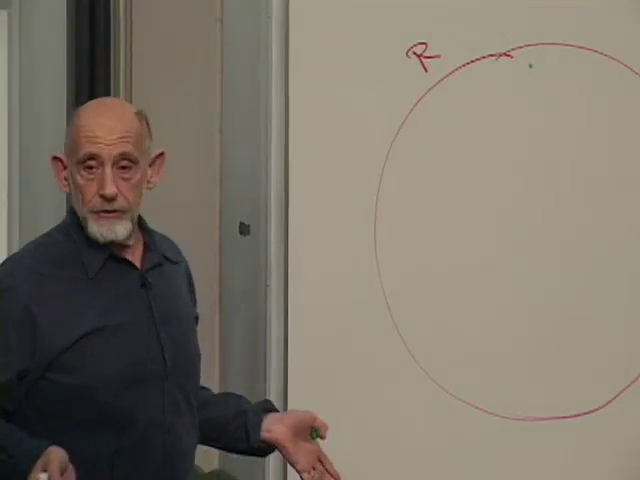
\includegraphics[width=0.74\textwidth]{lecture_09_figure_02.png}\caption{점입자 제어 계산:
\(p^2/(2m)=L^2/(2mR^2)=L^2/(2I)\).}\lectureframe{00:11:25}\label{fig:l09-sphere-rotor}\end{figure}

이처럼 문제가 없는 사례는 중요하다. 곡률 자체가 문제는 아니다. 문제는 곡률이 끈의 내부적인 양자적 크기와 결합할 때 나타난다.

\section{진공 상태의 끈은 점입자가 아니다}

열린 끈의 횡방향 좌표 하나를 생각하고 질량중심 성분을 빼자. 여기서 사용하는 진동자 전개는 개략적인 형태다:
\begin{equation}
  X(\sigma)-X_{\mathrm{cm}}
  \sim
  \sum_{n=1}^{\infty}
  \frac{a_n+a_n^\dagger}{\sqrt n}\cos(n\sigma).
  \label{eq:l09-mode-expansion}
\end{equation}
핵심 요소는 코사인 모드, 진동자 연산자, 그리고 \(1/\sqrt n\) 인자다. 크기 추정에는 정확한 정규화가 중요하지 않다.
\editorialnote{정확한 전개식에는 규약에 따라 달라지는 \(\alpha'\) 인자와 수치 상수, 그리고 진동자 표기법의 선택이 들어간다. 식 \eqref{eq:l09-mode-expansion}은 칠판에서 유도한 것과 마찬가지로 자외선 추정에 필요한 의존성만 남긴다.}

\begin{figure}[H]\centering
  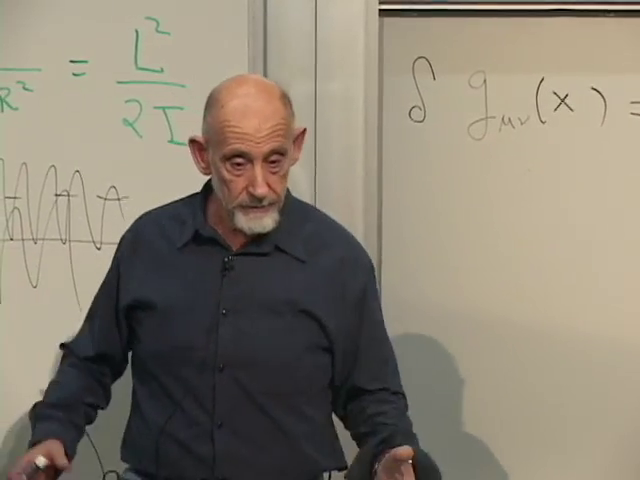
\includegraphics[width=0.78\textwidth]{lecture_09_figure_03.png}\caption{구조를 보여 주는 진동자 전개식과 이를 제곱해 얻는 이중합.}\lectureframe{00:15:20}\label{fig:l09-string-modes}\end{figure}

진동자 진공 상태에서 질량중심으로부터의 제곱 거리는
\begin{align}
  \expect{\bigl(X(\sigma)-X_{\mathrm{cm}}\bigr)^2}_0
  &\sim
  \sum_{n,m\geq1}
  \frac{\cos(n\sigma)\cos(m\sigma)}{\sqrt{nm}}\notag\\
  &\qquad\times
  \bra{0}(a_n+a_n^\dagger)\notag\\
  &\hspace{6em}\times(a_m+a_m^\dagger)\ket{0}.
  \label{eq:l09-size-double-sum}
\end{align}
대부분의 항은 사라진다. 소멸 연산자 두 개는 켓을 소멸시키고, 생성 연산자 두 개는 브라와 직교하는 상태를 만들며, 이 순서에서는 생성 연산자 뒤에 소멸 연산자가 오는 경우도 진공 기대값이 0이다. 살아남는 수축은
\begin{equation}
  \bra{0}a_n a_m^\dagger\ket{0}=\delta_{nm}.
  \label{eq:l09-vacuum-contraction}
\end{equation}

\begin{figure}[H]\centering
  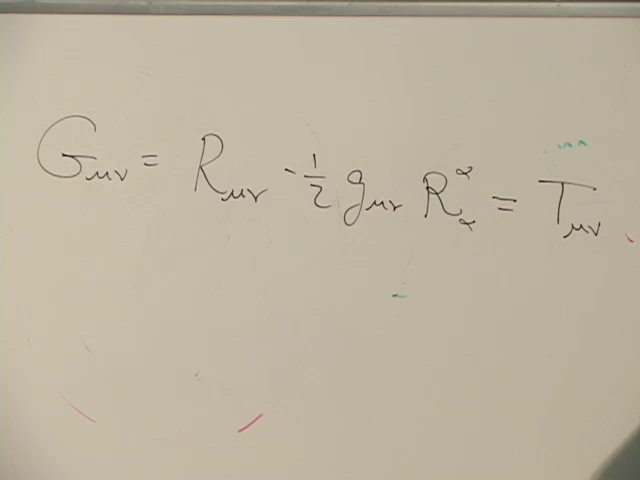
\includegraphics[width=0.74\textwidth]{lecture_09_figure_04.png}\caption{진공 수축으로 이중 진동자 합이 단일 합으로 줄어든다.}\lectureframe{00:20:10}\label{fig:l09-vacuum-contraction}\end{figure}

따라서
\begin{equation}
  \expect{\bigl(X(\sigma)-X_{\mathrm{cm}}\bigr)^2}_0
  \sim
  \sum_{n=1}^{\infty}\frac{\cos^2(n\sigma)}{n}.
  \label{eq:l09-size-single-sum}
\end{equation}
끈을 따라 일반적인 한 지점에서, 또는 \(\sigma\)에 대해 평균을 내면 \(\cos^2(n\sigma)\)는 대략 \(1/2\)가 된다. 모드 절단값을 \(N\)이라 하면,
\begin{equation}
  \expect{\bigl(X-X_{\mathrm{cm}}\bigr)^2}_{0,N}
  \sim
  \frac{1}{2}\sum_{n=1}^{N}\frac{1}{n}
  =\frac{1}{2}\log N+O(1).
  \label{eq:l09-logarithmic-size}
\end{equation}

\begin{figure}[H]\centering
  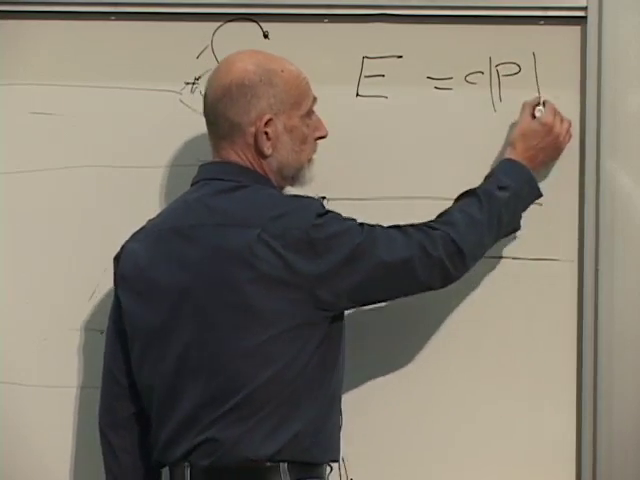
\includegraphics[width=0.72\textwidth]{lecture_09_figure_05.png}\caption{바닥 상태의 퍼짐을 좌우하는 조화급수에 이르는 칠판 유도.}\lectureframe{00:22:05}\label{fig:l09-harmonic-size}\end{figure}

예를 들어 처음 스물다섯 개 모드만 남기면 유한한 퍼짐을 가진 흐릿한 물체를 얻지만, 아직 연속적인 끈은 아니다. 절단값을 없애면 평균 제곱 퍼짐은 로그에 비례해 커진다. 이 결론을 평탄한 공간의 끈 이론이 비일관적이라는 증명으로 오해해서는 안 된다. 평탄한 공간에서는 질량중심 운동과 진동자 운동이 분리되며, 물리적 진폭에서의 섬세한 상쇄가 예상되는 국소성을 보존한다. 크기가 커진다는 것은 경고다. 곡률은 그 경고가 실제 실패로 이어지는지 알려 준다.

\section{내부 퍼짐이 기하를 바꿀 때}

끈을 구의 북극 근처에 놓자. 모든 진동자를 끈 상태에서는 방금 살펴본 점입자처럼 거동한다. 더 높은 모드를 허용하면 끈은 구면의 뚜껑 영역에 퍼진 요동하는 뒤엉킴이 된다. 질량중심은 여전히 구면을 따라 움직일 수 있지만, 회전 에너지에 들어가는 관성 모멘트의 대상은 이제 퍼져 있는 물체다.

구의 중심과 극을 지나는 축에 대해서는
\begin{equation}
  I=\int r_\perp^2\,dm,
  \label{eq:l09-extended-inertia}
\end{equation}
여기서 \(r_\perp\)는 끈의 한 요소와 축 사이의 수직 거리다. 궤도의 적도에 있는 점은 관련 지렛팔이 가장 길다. 축 쪽으로 처진 끈의 부분은 기여가 더 작다. 전체 질량을 고정하면 유효 관성 모멘트는 작아진다:
\begin{equation}
  I_{\mathrm{eff}}<mR^2.
  \label{eq:l09-inertia-reduction}
\end{equation}
따라서 회전 에너지는 더 작은 구면 위의 점물체 에너지처럼 보인다:
\begin{equation}
  E_{\mathrm{rot}}
  =\frac{L^2}{2I_{\mathrm{eff}}}
  \equiv \frac{L^2}{2mR_{\mathrm{eff}}^2},
  \qquad R_{\mathrm{eff}}<R.
  \label{eq:l09-effective-radius}
\end{equation}

\begin{classroomqa}\audiencequestion{끈이 더 넓은 영역으로 퍼지는데 관성 모멘트는 왜 0에 가까워져야 하나요? \lecturetimestamp{00:33:23}}\lecturerresponse{이는 퍼져 있는 원래 분포의 관성 모멘트가 즉시 0이 된다는 뜻이 아니라, 연속적인 거친 분해능 조정에 따른 유효 기술에 관한 말이다. 첫 번째 모드 띠는 점을 흐릿한 덩어리로 바꾸어 더 작은 구면 위에 있는 것처럼 움직이게 한다. 다음 띠는 각 덩어리 내부의 구조를 분해하고 같은 재규격화를 반복한다. 이 비교를 되풀이하면 유효 반지름은 안쪽으로 줄어든다.}\end{classroomqa}

\begin{figure}[H]
  \centering
  \includegraphics[width=0.72\textwidth]{lecture_09_figure_06.png}
  \medskip

  \begin{adjustbox}{max width=\linewidth}
  \begin{tikzpicture}[x=1cm,y=1cm,>=Latex]
    \draw[thick] (0,0) circle (2.15);
    \draw[dashed] (0,-2.55) -- (0,2.55);
    \draw[blue!65!black,thick]
      (-0.22,2.05)
      .. controls (-1.22,1.75) and (-1.52,1.08) .. (-1.06,0.44)
      .. controls (-0.55,-0.10) and (0.35,0.02) .. (1.10,0.68)
      .. controls (1.48,1.12) and (1.16,1.80) .. (0.20,2.05);
    \draw[red!70!black,dashed] (0,0) circle (1.25);
    \draw[->] (2.70,1.55) -- (4.05,1.55);
    \node[align=center] at (3.37,1.98) {add shorter\\modes};
    \draw[thick] (6.15,0) circle (1.25);
    \draw[dashed] (6.15,-1.65) -- (6.15,1.65);
    \draw[blue!65!black,thick]
      (6.00,1.18)
      .. controls (5.42,0.88) and (5.46,0.25) .. (6.02,-0.06)
      .. controls (6.46,-0.28) and (6.90,0.45) .. (6.28,1.18);
    \node at (0,-3.00) {sphere of radius \(R\)};
    \node at (6.15,-2.05) {effective radius \(R_{\mathrm{eff}}\)};
  \end{tikzpicture}
  \end{adjustbox}\caption{칠판에 그린 북극의 끈과 유효 반지름 논증을 깔끔하게 다시 그린 그림. 점선으로 표시한 안쪽 원은 유효 기하이지, 구 안에 들어 있는 두 번째 물리적 껍질이 아니다.}\lectureframe{00:35:15}\label{fig:l09-shrinking-sphere}\end{figure}

이는 재규격화군에 관한 진술이다. 유한한 절단값에서는 끈이 유한한 내부 분해능을 가진 덩어리로 보인다. 절단값을 높이면 그 덩어리의 역학이 바뀐다. 양의 곡률을 가진 구면에서는 모드 껍질을 하나씩 더 포함할 때마다 장거리 운동으로 추론하는 배경이 더 작아진다. 결과가 끝내 안정되지 않는다면 그 배경 위에는 절단값과 무관한 끈 이론이 존재하지 않는다.

\section{계량은 고정점에 도달해야 한다}

이제 구를 일반적인 표적 공간 계량 \(g_{\mu\nu}(x)\)으로 바꾸자. 진동자 모드의 얇은 로그 껍질에 대해 적분하면 계량은 국소적인 대칭 이계 텐서만큼 변한다. 이 변화는 평탄한 공간에서는 사라져야 하고, 계량의 두 미분을 포함하는 항에서 시작해야 한다. 선도 차수에서는 공변성에 따라 리치 텐서가 관련 후보로 남는다:
\begin{equation}
  \frac{\partial g_{\mu\nu}}{\partial\log\Lambda}
  =-C\,R_{\mu\nu}+\cdots ,
  \qquad C>0
  \label{eq:l09-ricci-flow}
\end{equation}
이는 기하학적 논증에서 사용한 조대화 방향을 따른 결과다. 따라서 양의 곡률은 구를 안쪽으로 수축시키며, 이는 요구된 바와 같다.
\editorialnote{정규화와 부호는 재규격화 매개변수가 자외선 쪽으로 증가하는지 적외선 쪽으로 증가하는지에 따라 달라진다. 통상적인 세계면 표기법에서 선도 차수의 계량 베타 함수는 \(\beta^g_{\mu\nu}=\alpha'R_{\mu\nu}+\cdots\)이다. 여기서 사용하는 불변적인 진술은 컷오프 독립성을 위해 베타 함수, 따라서 이 차수에서는 \(R_{\mu\nu}\)가 영이어야 한다는 것이다.}

\begin{figure}[H]\centering
  \includegraphics[width=0.76\textwidth]{lecture_09_figure_07.png}\caption{계량 변화는 리치 텐서의 음수에 비례하는 형태로 개략적으로 쓰고, 옆에는 매끄럽게 다듬어지는 곡선을 그렸다.}\lectureframe{00:43:00}\label{fig:l09-ricci-flow-board}\end{figure}

\begin{classroomqa}\audiencequestion{이 흐름 방정식에서 진동자 절단값 \(N\)은 어디에 나타나나요? \lecturetimestamp{00:43:38}}\lecturerresponse{그것이 척도 변수다. 포함하는 최고 모드가 바뀔 때 끈 크기 합은 로그에 따라 변하므로, 자연스러운 진화 매개변수는 \(\log N\), 또는 이와 동등하게 \(\log\Lambda\)이다. 식 \eqref{eq:l09-ricci-flow}은 모드의 로그 껍질 하나가 일으키는 미소 변화를 나타낸다.}\end{classroomqa}

허용 가능한 배경은 이 흐름의 고정점이다. 선도 차수에서는
\begin{equation}
  \boxed{R_{\mu\nu}=0.}
  \label{eq:l09-ricci-flat}
\end{equation}
리치 평탄하다고 해서 리만 텐서의 모든 성분이 영인 것은 아니다. 예를 들어 중력파는 \(R_{\mu\nu}=0\)를 만족하면서도 진공에서 영이 아닌 곡률을 가질 수 있다.

\subsection{같은 조건은 진공 아인슈타인 방정식이다}

통상적인 상수들을 생략하면 아인슈타인 방정식은 다음과 같다.
\begin{equation}
  G_{\mu\nu}
  \equiv
  R_{\mu\nu}-\frac12 g_{\mu\nu}R
  =T_{\mu\nu}.
  \label{eq:l09-einstein}
\end{equation}

\begin{figure}[H]\centering
  \includegraphics[width=0.78\textwidth]{lecture_09_figure_08.png}\caption{칠판에 적힌 아인슈타인 텐서와 응력 텐서.}\lectureframe{00:47:15}\label{fig:l09-einstein-board}\end{figure}

진공에서는 \(T_{\mu\nu}=0\)이다. \(D\) 시공간 차원에서 \begin{equation}
  0=g^{\mu\nu}G_{\mu\nu}
   =\left(1-\frac{D}{2}\right)R.
  \label{eq:l09-einstein-trace}
\end{equation}
\(D\neq2\)이면 \(R=0\)이고, 이를 \eqref{eq:l09-einstein}에 대입하면 \(R_{\mu\nu}=0\)를 얻는다. 따라서 끈의 컷오프 의존성이 사라지려면 진공 중력장 방정식이 성립해야 한다. 중력은 이론에 덧붙여진 것이 아니라, 일관성을 유지하기 위해 치러야 하는 대가로 나타났다.

\emph{진공}이라는 말은 아무 일도 일어나지 않는다는 뜻이 아니다. 해당 영역에 응력-에너지 원천이 없다는 뜻이다. 원천이 없는 맥스웰 방정식은 전자기파를 허용하고, 원천이 없는 아인슈타인 방정식은 중력파를 허용한다. 리치 텐서가 영이어도 기하학은 시간에 따라 변할 수 있다.

\begin{classroomqa}\audiencequestion{이 조건은 등각 불변성과 관련이 있나요?
\lecturetimestamp{00:52:20}}\lecturerresponse{그렇다. 다만 녹음에서는 질문의 일부가 잘려 있다. 관련 대칭은 양자 \emph{세계면}의 등각 불변성이다. 세계면 척도 변칙이 사라지도록 요구하면 계량 베타 함수가 0이 된다. 이를 시공간 자체의 등각 불변성을 요구하는 것과 혼동해서는 안 된다.}\end{classroomqa}

두 번째 일관성 조건도 있다. 세계면 등각 불변성은 임계 시공간 차원도 정한다. 초끈 이론에서는 10차원, 보손 끈 이론에서는 26차원이다. 따라서 리치 평탄성만으로 요구 조건 전체가 충족되지는 않지만, 아인슈타인 방정식을 가장 직접적으로 드러내는 부분은 바로 이것이다.

\section{사라진 차원이 아니라 콤팩트한 차원}

초끈 배경에는 공간 차원 9개와 시간 차원 1개가 있다. 거시적인 우리 세계에서 드러나는 큰 공간 방향은 3개뿐이므로, 나머지 공간 차원 6개는 숨겨져 있거나 보통의 척도에서 접근할 수 없게 되어 있어야 한다. 콤팩트화는 이 차원들을 실제 방향으로 남겨 두면서도 유한하고 작은 크기를 갖게 한다.

\begin{classroomqa}\audiencequestion{관찰자마다 다른 시계를 가지고 있다면 시간 차원이 둘 이상이라는 뜻인가요? \lecturetimestamp{00:56:59}}\lecturerresponse{아니다. 여러 시계는 하나의 시공간에서 좌표를 측정하는 여러 계측기일 뿐이며, 서로 독립적인 시간꼴 방향을 만들어 내지 않는다. 여기서 다루는 추가 차원은 공간 차원이다. 익숙한 양자 및 인과 구조로는 국소적인 시간 방향이 여러 개인 일관된 이론을 비슷하게 구성할 수 없으므로, 그런 가능성은 이 콤팩트화 모형에 포함되지 않는다.}\end{classroomqa}

자신들의 세계가 선이라고 믿는 생명체를 상상해 보자. 낮은 분해능에서는 앞뒤로만 움직일 수 있다. 하지만 충분히 강력한 현미경으로 보면 그 선은 매우 가느다란 원기둥으로 드러난다. 작은 생명체는 길이 방향뿐 아니라 원형 방향으로도 움직일 수 있다. 두 번째 방향은 처음부터 있었지만, 둘레가 너무 작아 거친 탐사로는 분해할 수 없었던 것이다.

\begin{figure}[H]\centering
  \includegraphics[width=0.78\textwidth]{lecture_09_figure_09.png}\caption{숨겨진 원형 방향을 따라 감기는 궤적이 있는 가느다란 원기둥.}\lectureframe{01:01:00}\label{fig:l09-hidden-cylinder}\end{figure}

원기둥은 위쪽과 아래쪽 가장자리를 서로 동일시한 띠로 나타낼 수 있다. 위쪽 가장자리로 나가면 같은 길이 좌표의 아래쪽 가장자리로 돌아온다. 어느 가장자리에도 물리적인 경계는 없다. 두 방향에도 같은 조작을 할 수 있다. 직사각형의 왼쪽과 오른쪽 가장자리를 동일시하고, 위쪽과 아래쪽 가장자리도 동일시하는 것이다. 그 결과가 2차원 토러스다.

\begin{figure}[H]
  \centering
  \includegraphics[width=0.76\textwidth]{lecture_09_figure_10.png}
  \medskip

  \begin{tikzpicture}[x=0.82cm,y=0.82cm,>=Latex]
    \draw[thick] (0,0) rectangle (4,2.15);
    \draw[blue!65!black,->] (0,2.48) -- (4,2.48);
    \draw[blue!65!black,->] (4,-0.34) -- (0,-0.34);
    \node at (2,-0.82) {one periodic direction};
    \draw[thick] (6.1,0) rectangle (10.1,2.15);
    \draw[blue!65!black,->] (6.1,2.48) -- (10.1,2.48);
    \draw[blue!65!black,->] (10.1,-0.34) -- (6.1,-0.34);
    \draw[red!70!black,->] (5.76,0) -- (5.76,2.15);
    \draw[red!70!black,->] (10.44,2.15) -- (10.44,0);
    \node at (8.1,-0.82) {two periodic directions};
  \end{tikzpicture}\caption{칠판의 판 모양 그림과 기본 영역을 깔끔하게 다시 그린 그림. 한 쌍의 가장자리를 동일시하면 원기둥이 되고, 두 쌍을 모두 동일시하면 토러스가 된다.}\lectureframe{01:04:40}\label{fig:l09-periodic-identification}\end{figure}

토러스는 먼저 위상 공간이며, 3차원 공간 안의 도넛 모양 곡면인 것은 그다음이다. 토러스를 한 번 자르면 원기둥이 되고, 가장자리 동일시를 기억해 두면 한 번 더 잘라 직사각형이 된다. 이 직사각형에 평탄한 계량을 줄 수 있으므로, 이렇게 얻은 평탄 토러스는 국소적으로 리만 곡률이 0이며 당연히 리치 평탄하다.

직사각형 위의 직선 궤적은 동일시된 가장자리를 지나서도 곧게 이어진다. 기울기가 두 주기의 유리수 비라면 궤적은 결국 닫힌다. 그 비가 무리수라면 궤적은 닫히지 않고 토러스 위를 조밀하게 채운다.

\begin{figure}[H]\centering
  \includegraphics[width=0.76\textwidth]{lecture_09_figure_11.png}\caption{기본 영역 안의 반복되는 직선 선분은 토러스 위에서 중단 없이 이어지는 하나의 궤적을 나타낸다.}\lectureframe{01:11:00}\label{fig:l09-torus-trajectory}\end{figure}

고차원 토러스도 같은 방식으로 만든다. 서로 마주 보는 각 면 쌍을 동일시한 정육면체는 3차원 토러스이고, 6개의 콤팩트 차원은 6차원 토러스로 모형화할 수 있다. 이 물체들을 보통의 3차원 공간 안에 모두 끼워 넣으려 해서는 안 된다. 면을 동일시하는 설명만으로 내재적으로 완전하게 기술할 수 있다.

\begin{classroomqa}\audiencequestion{추가 차원은 반드시 다시 자기 자신과 이어져야 하나요?
\lecturetimestamp{01:15:03}}\lecturerresponse{정리상 반드시 그런 것은 아니다. 비콤팩트 차원일 수도 있지만, 그러면 보통 관측되는 장거리 세계에 또 하나의 큰 방향으로 나타날 것이다. 추가 차원이 없는 것처럼 보이는 현상과 양립하는 가장 간단한 방법은 콤팩트하게 만드는 것이다. 자연이 특정한 콤팩트화를 선택하는 이유는 별개의 동역학적 질문이다.}\end{classroomqa}

\begin{classroomqa}\audiencequestion{보이지 않는 차원이 이런 식으로 말린 보통의 공간 방향이라고 가정하는 이유는 무엇인가요? 완전히 다른 것일 수도 있지 않나요? \lecturetimestamp{01:15:51}}\lecturerresponse{이 가설이 자연을 기술하는 유일한 방식이라고 증명되었기 때문이 아니라, 명확하고 풀 수 있는 가설이기 때문이다. 콤팩트 공간 다양체를 이용하면 일관된 사례를 구성하고 그 스펙트럼을 계산할 수 있다. 더 이국적인 가능성도 같은 일을 해내야 받아들일 근거를 얻는다.}\end{classroomqa}

\begin{classroomqa}\audiencequestion{익숙한 도넛 모양 토러스에서의 거리는 직사각형에서의 거리처럼 보이지 않습니다. 어떤 기하를 뜻하나요?
\lecturetimestamp{01:18:11}}\lecturerresponse{\emph{토러스}라는 말은 동일시 방법을 정할 뿐, 유일한 계량을 정하지는 않는다. 공간에 끼워 넣은 도넛은 3차원 공간에서 유도된 곡률 있는 계량을 갖는다. 주기적으로 가장자리를 동일시한 직사각형은 평탄한 계량을 갖는다. 두 공간은 위상은 같지만 기하는 다르다. 간단한 콤팩트화에서 말하는 것은 평탄한 쪽이다.}\end{classroomqa}

\section{평탄 토러스의 모양 매개변수}

평탄한 2차원 토러스도 하나로 정해지지 않는다. 기본 평행사변형에는 전체 면적, 종횡비, 그리고 전단이 있다. 이 매개변수들을 바꾸면 위상은 그대로지만 거리가 달라지고, 따라서 스펙트럼도 달라진다.

\begin{figure}[H]
  \centering
  \includegraphics[width=0.74\textwidth]{lecture_09_figure_12.png}
  \medskip

  \begin{tikzpicture}[x=0.9cm,y=0.9cm,>=Latex]
    \draw[thick] (0,0) rectangle (3.4,2.1);
    \draw[<->] (0,-0.35) -- node[below] {\(L_1\)} (3.4,-0.35);
    \draw[<->] (-0.35,0) -- node[left] {\(L_2\)} (-0.35,2.1);
    \draw[thick] (5.4,0) -- (8.8,0) -- (9.7,2.1) -- (6.3,2.1) -- cycle;
    \draw[dashed] (5.4,0) -- (6.3,2.1);
    \draw[->] (5.75,2.48) -- node[above] {shear} (6.45,2.48);
    \node at (1.7,-1.00) {area and aspect ratio};
    \node at (7.55,-1.00) {complex structure};
  \end{tikzpicture}\caption{토러스 모듈라이를 설명하는 데 사용하는 직사각형 및 전단된 기본 영역.}\lectureframe{01:23:00}\label{fig:l09-torus-moduli}\end{figure}

2차원 토러스에서는 모양을 복소수 \(\tau=\tau_1+i\tau_2\) 하나로 나타내면 편리하다. 실수부는 전단을 기록하고, 전체 척도를 분리한 뒤 허수부는 종횡비를 기록한다. 두 기본 주기를 서로 바꾸거나 정수 기저를 바꾸면, 겉보기에 다른 평행사변형이 같은 토러스를 나타낼 수 있다.

\begin{classroomqa}\audiencequestion{동일시하기 전에 한쪽 가장자리를 뒤집으면 어떻게 되나요? \lecturetimestamp{01:24:20}}\lecturerresponse{위상이 달라진다. 반사해서 동일시하면 보통의 토러스가 아니라 비가향 곡면인 클라인 병이 된다.}\end{classroomqa}

\begin{classroomqa}\audiencequestion{가장자리를 따라 비틀림이 일정하지 않으면 어떻게 되나요?
\lecturetimestamp{01:25:01}}\lecturerresponse{매끄럽고 일정하지 않은 변형은 기본 영역의 계량으로 옮겨 담을 수 있다. 위상적 동일시와 기하학적 자료는 구분해서 다뤄야 한다. 붙이는 방식을 바꾸면 위상이 달라질 수 있지만, 거리를 매끄럽게 바꾸면 계량이 달라진다.}\end{classroomqa}

\editorialnote{평탄한 2차원 토러스에서 면적은 가장 단순한 칼러 모듈러스이며, \(\tau\)는 복소구조 모듈러스다. 연속적인 전단은 \(\tau\)의 일부다. 반면 데ーン 비틀기는 이산적인 사상류 연산으로, \(\tau\mapsto\tau+1\)로 나타낸다. 이것 자체가 연속 모듈러스인 것은 아니다. 이는 칠판 논의에서 의도적으로 비격식적으로 사용한 용어를 더 정확히 다듬은 것이다.}

평탄 토러스는 일관성 조건을 즉시 만족하므로 유용하지만, 대칭성이 지나치게 커서 현실적인 입자물리학 모형에는 적합하지 않다. 칼라비--야우 다양체처럼 더 복잡한 리치 평탄 공간은 더 풍부한 콤팩트화를 제공한다. 그 구체적인 구성은 이 논의의 범위를 벗어나지만, 기본 원리는 같다.

\section{스펙트럼에서 콤팩트 원 읽어내기}

휴식 후에는 콤팩트 공간을 둘레가 \(2\pi R\)인 원 하나로 줄여 보자. 파동함수는 원을 한 바퀴 돈 뒤 단일값이어야 한다:
\begin{equation}
  e^{ip_c(x+2\pi R)/\hbar}=e^{ip_cx/\hbar}.
\end{equation}
따라서
\begin{equation}
  p_cR=n\hbar,
  \qquad
  p_c=\frac{n\hbar}{R},
  \qquad n\in\mathbb Z.
  \label{eq:l09-kk-momentum}
\end{equation}

\begin{figure}[H]\centering
  \includegraphics[width=0.74\textwidth]{lecture_09_figure_13.png}\caption{\(2\pi R\)와 양자화된 운동량 \(p_c=n\hbar/R\).}\lectureframe{01:32:15}\label{fig:l09-kk-board}\end{figure}

전체 시공간에서 질량이 없는 입자의 경우,
\begin{equation}
  E=c|\mathbf P|.
  \label{eq:l09-massless-dispersion}
\end{equation}

\begin{figure}[H]\centering
  \includegraphics[width=0.70\textwidth]{lecture_09_figure_14.png}\caption{콤팩트 운동량을 저차원 질량으로 재해석하는 데 쓰이는 질량 없는 입자의 분산 관계.}\lectureframe{01:33:45}\label{fig:l09-massless-board}\end{figure}

운동량을 비콤팩트 성분과 콤팩트 성분으로 나누고 \(c=\hbar=1\)로 놓자:
\begin{equation}
  E^2=\mathbf p_{\mathrm{large}}^2+\frac{n^2}{R^2}.
  \label{eq:l09-kk-dispersion}
\end{equation}
콤팩트 방향을 분해할 수 없는 관찰자는 이를 \(E^2=\mathbf p_{\mathrm{large}}^2+m^2\)와 비교하여 질량 탑을 추론한다:
\begin{equation}
  m_n=\frac{|n|}{R}.
  \label{eq:l09-kk-masses}
\end{equation}
\(n\)의 두 부호는 양의 에너지를 갖는 반대 방향의 콤팩트 운동량을 나타내며, 양의 질량과 음의 질량을 뜻하지 않는다. 따라서 간격 \(1/R\)을 분광학적으로 측정하면 반지름을 알아낼 수 있다. 이것이 칼루차--클라인 기작이다. 숨겨진 방향의 운동량이 보이는 차원에서는 질량으로 나타난다.

\section{감김 상태가 스펙트럼을 완성한다}

닫힌 끈에는 점입자에게 없는 가능성이 있다. 원을 감을 수 있다는 것이다. 감김수가 \(w\)라면 끈은 콤팩트 방향을 \(w\)번 돈 뒤에야 닫힌다. 끈의 길이는 \(2\pi |w|R\)이므로 장력에 따라 에너지가 생긴다:
\begin{equation}
  m_w
  =2\pi T\,|w|R
  =\frac{|w|R}{\alpha'}.
  \label{eq:l09-winding-mass}
\end{equation}
강의에서는 \(\alpha'=1\)인 단위를 선택하여 다음처럼 쓴다:
\begin{equation}
  m_w=|w|R.
  \label{eq:l09-winding-lecture-units}
\end{equation}
\(w\)의 양수와 음수는 원을 도는 방향이 서로 반대임을 나타낸다.

\begin{figure}[H]\centering
  \includegraphics[width=0.76\textwidth]{lecture_09_figure_15.png}\caption{칠판에 표시한 콤팩트 반지름과 함께 콤팩트 원기둥을 감은 닫힌 끈.}\lectureframe{01:39:45}\label{fig:l09-winding-board}\end{figure}

따라서 콤팩트 원은 서로 보완적인 두 탑을 만든다:
\begin{equation}
  m_n=\frac{|n|}{R},
  \qquad
  m_w=\frac{|w|R}{\alpha'}.
  \label{eq:l09-two-towers}
\end{equation}
\(R\)가 클 때 운동량 준위의 간격은 촘촘하고 감김 상태는 무겁다. \(R\)가 작을 때는 운동량 준위의 간격이 넓고 감김 상태는 가볍다.

\begin{figure}[H]\centering
  \begin{tikzpicture}[x=1cm,y=0.9cm,>=Latex]
    \draw[->] (0,0) -- (0,4.7) node[above] {\(m\)};
    \foreach \y/\lab in {0/0,1.1/{1/R},2.2/{2/R},3.3/{3/R},4.4/{4/R}} {
      \draw (-0.16,\y) -- (0.16,\y);
      \node[left] at (-0.22,\y) {\(\lab\)};
    }
    \node at (0,-0.62) {momentum};
    \draw[<->,very thick,blue!65!black] (2.05,2.15) -- (4.05,2.15)
      node[midway,above] {\(R\leftrightarrow\alpha'/R\)};
    \draw[->] (6.1,0) -- (6.1,4.7) node[above] {\(m\)};
    \foreach \y/\lab in {0/0,1.1/{R/\alpha'},2.2/{2R/\alpha'},3.3/{3R/\alpha'},4.4/{4R/\alpha'}} {
      \draw (5.94,\y) -- (6.26,\y);
      \node[right] at (6.32,\y) {\(\lab\)};
    }
    \node at (6.1,-0.62) {winding};
  \end{tikzpicture}\caption{반지름을 끈 단위로 역수화하면 운동량 탑과 감김 탑이 서로 바뀐다.}\label{fig:l09-dual-mass-towers}\end{figure}

\section{T-쌍대성: 작은 원과 큰 원은 같은 물리학이다}

두 탑은 다음 변환으로 서로 바뀐다:
\begin{equation}
  R\longleftrightarrow\frac{\alpha'}{R},
  \qquad
  n\longleftrightarrow w.
  \label{eq:l09-t-duality}
\end{equation}
칠판에서 사용한 단위에서는 \(\alpha'=1\)이므로, 이는 간단히 \(R\leftrightarrow1/R\)가 된다. 자기쌍대 반지름 \(R=\sqrt{\alpha'}\)에서는 운동량과 감김의 척도가 일치한다.

\begin{figure}[H]\centering
  \includegraphics[width=0.74\textwidth]{lecture_09_figure_16.png}\caption{반지름이 자기쌍대 척도를 지날 때 칠판에서 비교한 성긴 질량 준위와 촘촘한 질량 준위.}\lectureframe{01:43:00}\label{fig:l09-duality-board}\end{figure}

기본 질량 공식들이 서로 바뀐다는 것은 결과의 겉으로 드러난 일부에 불과하다. 닫힌 끈의 진동자 상태와 산란 진폭도 일관되게 대응된다. 끈 척도보다 작은 원은 계속 더 작아지는 새로운 기하가 아니라, 더 큰 쌍대 원으로 동등하게 기술된다. 점입자에는 운동량 모드만 있고 감김 모드는 없으므로 이런 대응을 만들 수 없다.

\begin{classroomqa}\audiencequestion{수직 방향과 수평 방향을 서로 바꾸는 것과 같은 뜻인가요? \lecturetimestamp{01:44:38}}\lecturerresponse{아니다. 서로 다른 두 양자수, 즉 원을 따라 도는 운동량과 닫힌 끈이 원을 감는 횟수를 서로 바꾸는 것이다. 이와 동시에 반지름을 역수화해야 한다.}\end{classroomqa}

\begin{classroomqa}\audiencequestion{\(R<\sqrt{\alpha'}\)와 \(R>\sqrt{\alpha'}\)에서 비교하는 기술은 보손에만 해당하나요, 페르미온에도 해당하나요?
\lecturetimestamp{01:46:30}}\lecturerresponse{이 쌍대성은 이를 설명하기 위해 사용한 단순한 보손 질량 탑만의 대칭이 아니라, 콤팩트화된 끈 이론 전체의 대칭이다. 각 부문의 구체적인 대응은 이론에 따라 다르지만, 작은 원과--큰 원의 동등성은 특정 입자 종류에 한정되지 않는다.}\end{classroomqa}

\begin{classroomqa}\audiencequestion{비교하는 두 상태는 열린 끈인가요, 닫힌 끈인가요? \lecturetimestamp{01:47:32}}\lecturerresponse{닫힌 끈 상태다. 자유롭게 전파되는 닫힌 끈은 콤팩트 원을 감을 수 있다. 끝점이 자유로운 보통의 열린 끈은 같은 보존 감김수를 갖지 않는다.}\end{classroomqa}\editorialnote{더 완전한 열린 끈 설명에서는 T-쌍대성이 노이만 경계 조건과 디리클레 경계 조건을 서로 바꾸고 D-막을 도입한다. 그래서 열린 끈의 T-쌍대성은 닫힌 끈의 감김 공식을 단순히 그대로 옮기는 것보다 풍부하다.}

\begin{classroomqa}\audiencequestion{이 대응은 블랙홀 지평선 근처에서 공간과 시간이 서로 바뀌는 것과 비슷한가요? \lecturetimestamp{01:48:00}}\lecturerresponse{아니다. 지평선 좌표와 인과적 성격은 다른 문제다. 여기서 두 기술은 하나의 콤팩트한 공간 원과 그 운동량 부문 및 감김 부문의 교환을 다룬다.}\end{classroomqa}

\begin{classroomqa}\audiencequestion{이로써 최소 길이를 도입해 짧은 거리 자기 에너지 문제를 해결하나요? \lecturetimestamp{01:48:35}}\lecturerresponse{끈 척도보다 작은 반지름은 서로 동등하지 않은 새로운 원 배경을 정의하지 않는다는 것을 보여 준다. 자기쌍대점을 지나 \(R\)를 줄이면 쌍대 반지름은 커진다. 이는 임의로 작은 원 기하를 탐사하지 못하게 하는 정밀한 끈 이론적 제약이다. 다만 이를 모든 가능한 거리 개념에 보편적인 엄격한 하한이 있다는 주장으로 확대해서는 안 된다.}\end{classroomqa}

\section{감김 부문을 생략할 수 없는 이유}

\begin{classroomqa}
\audiencequestion{감기지 않은 끈만으로 이론을 정의하고 감김 상태는 제외할 수 있을까요? \lecturetimestamp{01:48:56}}
\lecturerresponse{아니요. 닫힌 끈의 상호작용으로 감김 상태가 생성됩니다. 감기지 않은 고리를 늘여 콤팩트한 방향을 감싸게 하면, 한 구간은 원을 한쪽 방향으로 돌고 다른 구간은 반대 방향으로 돕니다. 순감김수는 여전히 0입니다. 그러면 재접속으로 고리가 감김수가 \(+1\)인 닫힌 끈 하나와 \(-1\)인 닫힌 끈 하나로 나뉠 수 있습니다. 이 두 끈은 서로 멀어질 수 있으므로, 초기 상태에 감김이 전혀 없더라도 감김 상태는 스펙트럼에 포함되어야 합니다.}
\end{classroomqa}

\begin{figure}[H]
\centering
  \includegraphics[width=0.74\textwidth]{lecture_09_figure_17.png}
  \caption{재접속 전, 콤팩트한 방향을 감싸도록 배치한 늘어난 영감김 고리.}
  \lectureframe{01:50:30}
  \label{fig:l09-winding-pair-before}
\end{figure}

\begin{figure}[H]
  \centering
  \includegraphics[width=0.72\textwidth]{lecture_09_figure_18.png}
  \medskip

  \begin{tikzpicture}[x=0.9cm,y=0.9cm,>=Latex]
    \draw[thick] (0,0) ellipse (1.0 and 1.55);
    \draw[blue!65!black,thick]
      (0.08,1.35) .. controls (2.0,1.15) and (2.0,-1.15) .. (0.08,-1.35);
    \draw[red!70!black,thick]
      (-0.08,-1.35) .. controls (-2.0,-1.15) and (-2.0,1.15) .. (-0.08,1.35);
    \node at (0,-2.15) {net \(w=0\)};
    \draw[->,thick] (2.45,0) -- (3.75,0) node[midway,above] {split};
    \draw[thick] (5.05,0.62) ellipse (0.68 and 1.02);
    \draw[blue!65!black,very thick,->]
      (5.05,1.64) arc[start angle=90,end angle=-250,x radius=0.68,y radius=1.02];
    \node at (5.05,-0.82) {\(w=+1\)};
    \draw[thick] (7.45,0.62) ellipse (0.68 and 1.02);
    \draw[red!70!black,very thick,<-]
      (7.45,1.64) arc[start angle=90,end angle=-250,x radius=0.68,y radius=1.02];
    \node at (7.45,-0.82) {\(w=-1\)};
  \end{tikzpicture}
  \caption{칠판에 그린 서로 분리된 감긴 고리와 감김--반감김 쌍 생성의 깔끔한 재구성. 전체 감김수는 여전히 0이다.}
  \lectureframe{01:51:30}
  \label{fig:l09-winding-pair-after}
\end{figure}

\begin{classroomqa}
\audiencequestion{감김 쌍을 생성하려면 추가 에너지가 필요한가요?
\lecturetimestamp{01:52:11}}
\lecturerresponse{네. 끈을 늘이는 데 장력 에너지가 들고, 최종 상태의 감긴 끈들은 \eqref{eq:l09-winding-mass}에 주어진 질량을 가집니다. 충분히 에너지가 큰 충돌이라면 이 쌍을 생성할 수 있습니다. 이는 관련 보존 전하를 보존하면서 충돌로 입자와 반입자를 생성할 수 있는 것과 같습니다.}
\end{classroomqa}

\section{끈 배경의 형태를 소리로 알아낼 수 있을까?}

일반적인 콤팩트화 입자 이론에서는 칼루차--클라인 스펙트럼의 간격으로부터 반지름을 추론할 수 있습니다. 즉, 정상 모드를 통해 콤팩트 공간의 형태를 알아내려 합니다. 끈 이론에서는 역문제가 더 미묘해집니다. 운동량 모드는 \(1/R\)를, 감김 모드는 \(R/\alpha'\)를 반영하며, 두 모드를 서로 바꾸어도 전체 스펙트럼은 변하지 않습니다. 점입자 기하학에서 서로 다른 것으로 여기는 두 반지름은 이중 변수로 표현한 하나의 끈 배경입니다.

따라서 이 강의는 하나의 경로를 따라 예고했던 두 결론에 모두 도달했습니다. 자외선 영역의 일관성을 위해 표적 계량은 진공 아인슈타인 방정식을 만족해야 하므로 중력은 불가피합니다. 이어지는 콤팩트화는 숨은 기하를 입자 스펙트럼으로 바꾸지만, 감김 상태 때문에 그 스펙트럼만으로는 끈 척도 아래의 고전적 반지름을 유일하게 정할 수 없습니다. 일관성은 허용되는 기하가 무엇인지 정할 뿐 아니라, T 이중성을 통해 무엇을 서로 다른 기하로 볼 것인지도 바꿉니다.
